\documentclass[11pt]{article}
\usepackage[margin=1in]{geometry}
\usepackage{amsmath,amssymb}
\usepackage{tikz}
\usepackage{pgfplots}
\usepackage{booktabs}
\usepackage{xcolor}
\usepackage{float}

\usetikzlibrary{patterns,calc,arrows.meta,positioning}
\pgfplotsset{compat=1.18}

% Brand colors
\definecolor{garnet}{HTML}{73000A}
\definecolor{atlantic}{HTML}{466A9F}
\definecolor{congaree}{HTML}{1F414D}
\definecolor{horseshoe}{HTML}{65780B}
\definecolor{rose}{HTML}{CC2E40}
\definecolor{black90}{HTML}{363636}
\definecolor{black70}{HTML}{5C5C5C}
\definecolor{black50}{HTML}{A2A2A2}
\definecolor{black30}{HTML}{C7C7C7}
\definecolor{honeycomb}{HTML}{A49137}

\newcommand{\degC}{$^\circ$C}
\newcommand{\unit}[1]{\,\mathrm{#1}}

\title{\textbf{Transient Cooling Analysis:\\Water in Insulated Cylinder Enclosure}}
\author{J.C. Vaught}
\date{\today}

\begin{document}
\maketitle

\section{Problem Statement}

A volume of water initially at $T_0 = 90$\degC{} is contained in a cylinder inside a plywood enclosure. We want to determine how the water temperature decreases over time as heat is lost to the ambient environment at $T_\infty = 20$\degC.

\begin{table}[H]
\centering
\caption{System parameters}
\begin{tabular}{lll}
\toprule
\textbf{Parameter} & \textbf{Symbol} & \textbf{Value} \\
\midrule
Cylinder diameter & $D$ & 25 cm \\
Cylinder length & $L$ & 30 cm \\
Water volumes analyzed & $V$ & 5, 10, 15 liters \\
Initial temperature & $T_0$ & 90\degC \\
Ambient temperature & $T_\infty$ & 20\degC \\
\midrule
Water density & $\rho$ & 1000 kg/m$^3$ \\
Water specific heat & $c_p$ & 4186 J/(kg$\cdot$K) \\
\bottomrule
\end{tabular}
\end{table}

\section{Governing Equation}

Using the lumped capacitance model (assuming uniform water temperature):

\begin{equation}
    m c_p \frac{dT}{dt} = -\frac{T - T_\infty}{R_{total}}
\end{equation}

where:
\begin{itemize}
    \item $m$ = water mass [kg]
    \item $c_p$ = specific heat capacity [J/(kg$\cdot$K)]
    \item $R_{total}$ = total thermal resistance [K/W] (temperature-dependent due to radiation)
\end{itemize}

For constant $R_{total}$, the analytical solution is:
\begin{equation}
    T(t) = T_\infty + (T_0 - T_\infty) e^{-t/\tau}
\end{equation}

where the \textbf{time constant} is:
\begin{equation}
    \tau = R_{total} \cdot m \cdot c_p = R_{total} \cdot C
\end{equation}

\section{Thermal Capacitance}

\begin{table}[H]
\centering
\caption{Thermal capacitance for different water volumes}
\begin{tabular}{cccc}
\toprule
\textbf{Volume [L]} & \textbf{Mass [kg]} & \textbf{$C = mc_p$ [kJ/K]} & \textbf{Energy to cool [kJ]} \\
\midrule
5 & 5.0 & 20.9 & 1,465 \\
10 & 10.0 & 41.9 & 2,930 \\
15 & 15.0 & 62.8 & 4,395 \\
\bottomrule
\end{tabular}
\end{table}

The energy required to cool from 90\degC{} to 20\degC:
\begin{equation}
    E = m c_p \Delta T = m \times 4186 \times 70 \unit{J}
\end{equation}

\section{Time Constant Analysis}

From the steady-state analysis, the thermal resistance is approximately:
\begin{equation}
    R_{total} \approx 0.75 - 0.95 \unit{K/W}
\end{equation}

(varies with temperature due to radiation dependence)

\begin{table}[H]
\centering
\caption{Time constants and cooling times}
\begin{tabular}{ccccc}
\toprule
\textbf{Volume} & \textbf{$\tau$} & \textbf{$T$ at $t=\tau$} & \textbf{Time to 60\degC} & \textbf{Time to 40\degC} \\
{[L]} & [hours] & [\degC] & [hours] & [hours] \\
\midrule
5 & 5.5 & 45.8 & 2.6 & 6.3 \\
10 & 10.0 & 45.8 & 5.2 & 12.6 \\
15 & 14.5 & 45.8 & 7.9 & 18.9 \\
\bottomrule
\end{tabular}
\end{table}

\textbf{Key insight}: The time constant $\tau$ scales linearly with water mass. Doubling the water volume doubles the cooling time.

\section{Temperature vs. Time}

\begin{figure}[H]
\centering
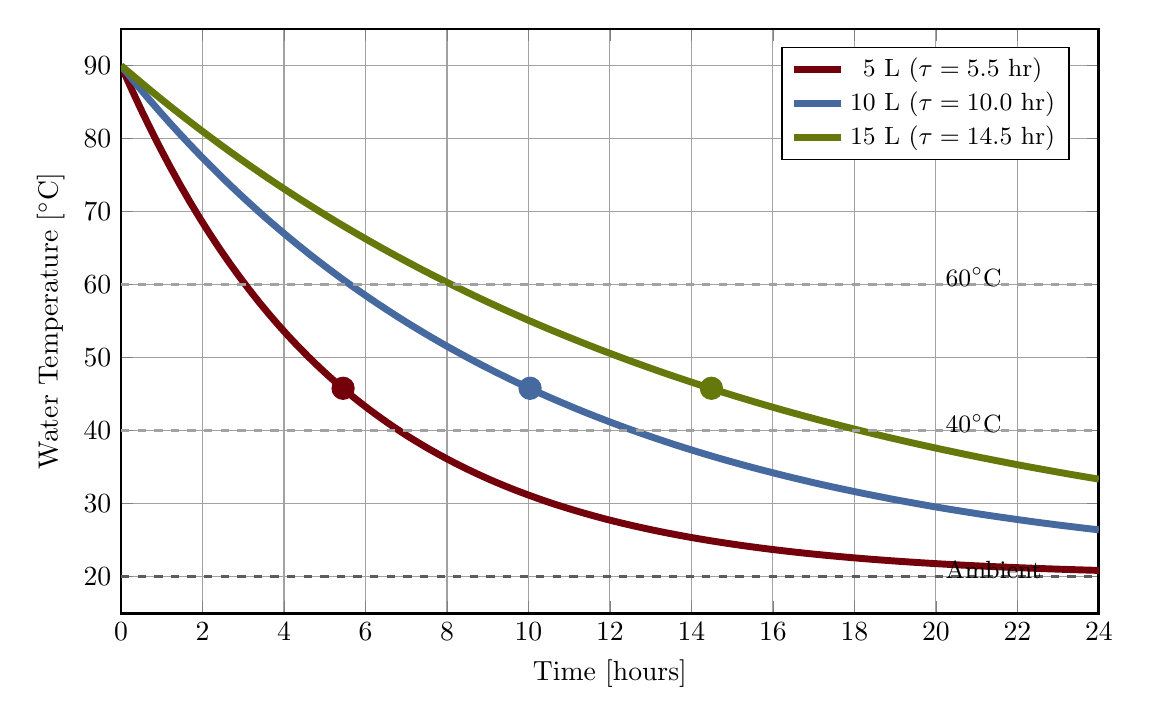
\begin{tikzpicture}
\begin{axis}[
    width=14cm,
    height=9cm,
    xlabel={Time [hours]},
    ylabel={Water Temperature [\degC]},
    xmin=0, xmax=24,
    ymin=15, ymax=95,
    grid=both,
    grid style={line width=0.2pt, draw=black30},
    major grid style={line width=0.4pt, draw=black50},
    legend pos=north east,
    legend style={font=\small},
    axis line style={line width=1pt},
]

% 5 liters - exponential decay with tau = 5.45 hours
\addplot[
    domain=0:24,
    samples=100,
    line width=2.5pt,
    color=garnet,
] {20 + 70*exp(-x/5.45)};
\addlegendentry{5 L ($\tau = 5.5$ hr)}

% 10 liters - tau = 10.04 hours
\addplot[
    domain=0:24,
    samples=100,
    line width=2.5pt,
    color=atlantic,
] {20 + 70*exp(-x/10.04)};
\addlegendentry{10 L ($\tau = 10.0$ hr)}

% 15 liters - tau = 14.49 hours
\addplot[
    domain=0:24,
    samples=100,
    line width=2.5pt,
    color=horseshoe,
] {20 + 70*exp(-x/14.49)};
\addlegendentry{15 L ($\tau = 14.5$ hr)}

% Reference lines
\addplot[dashed, line width=1pt, black50] coordinates {(0,60) (24,60)};
\node[right, font=\small] at (axis cs:20,61) {60\degC};

\addplot[dashed, line width=1pt, black50] coordinates {(0,40) (24,40)};
\node[right, font=\small] at (axis cs:20,41) {40\degC};

\addplot[dashed, line width=1pt, black70] coordinates {(0,20) (24,20)};
\node[right, font=\small] at (axis cs:20,21) {Ambient};

% Time constant markers (T = 45.8°C at t = tau)
\addplot[only marks, mark=*, mark size=4pt, color=garnet] coordinates {(5.45, 45.8)};
\addplot[only marks, mark=*, mark size=4pt, color=atlantic] coordinates {(10.04, 45.8)};
\addplot[only marks, mark=*, mark size=4pt, color=horseshoe] coordinates {(14.49, 45.8)};

\end{axis}
\end{tikzpicture}
\caption{Water temperature vs. time for different volumes. Dots mark the time constant $\tau$ where $T = 45.8$\degC{} (36.8\% of $\Delta T$ remaining).}
\end{figure}

\section{Heat Loss Rate vs. Time}

\begin{figure}[H]
\centering
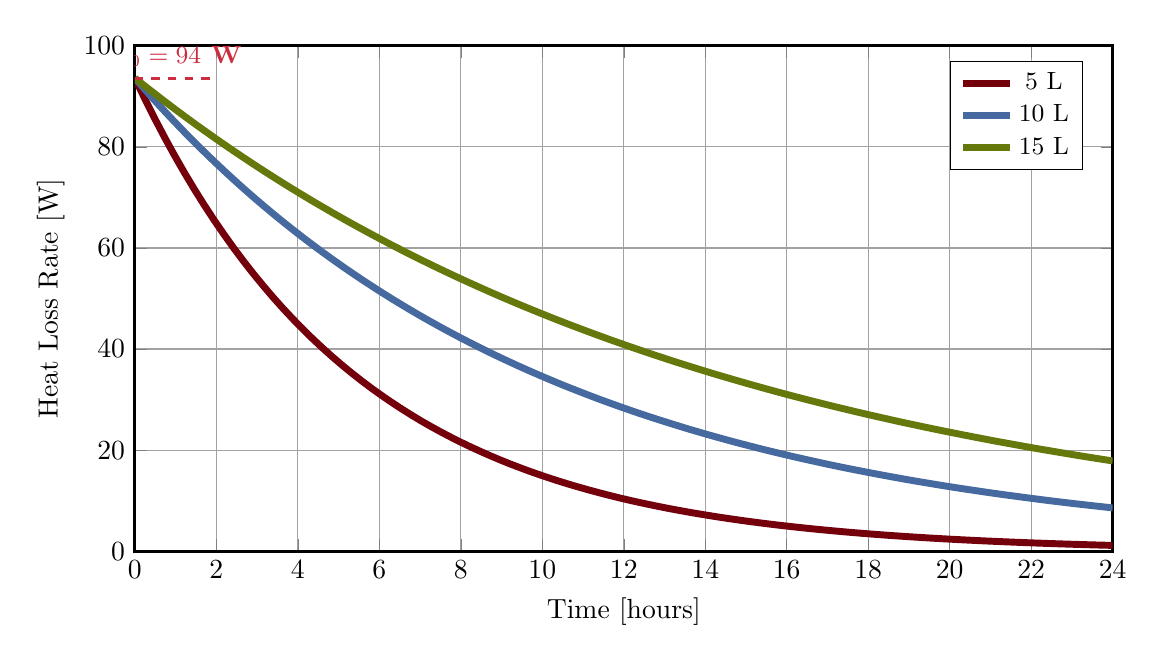
\begin{tikzpicture}
\begin{axis}[
    width=14cm,
    height=8cm,
    xlabel={Time [hours]},
    ylabel={Heat Loss Rate [W]},
    xmin=0, xmax=24,
    ymin=0, ymax=100,
    grid=both,
    grid style={line width=0.2pt, draw=black30},
    major grid style={line width=0.4pt, draw=black50},
    legend pos=north east,
    legend style={font=\small},
    axis line style={line width=1pt},
]

% Heat loss Q = (T - T_amb) / R_total
% Q(t) = (T_0 - T_amb) * exp(-t/tau) / R_total = Q_0 * exp(-t/tau)
% Q_0 = 70 / 0.75 ≈ 93 W

% 5 liters
\addplot[
    domain=0:24,
    samples=100,
    line width=2.5pt,
    color=garnet,
] {93.6*exp(-x/5.45)};
\addlegendentry{5 L}

% 10 liters
\addplot[
    domain=0:24,
    samples=100,
    line width=2.5pt,
    color=atlantic,
] {93.6*exp(-x/10.04)};
\addlegendentry{10 L}

% 15 liters
\addplot[
    domain=0:24,
    samples=100,
    line width=2.5pt,
    color=horseshoe,
] {93.6*exp(-x/14.49)};
\addlegendentry{15 L}

% Initial heat loss marker
\addplot[dashed, line width=1pt, rose] coordinates {(0,93.6) (2,93.6)};
\node[above, rose, font=\small\bfseries] at (axis cs:1,93.6) {$Q_0 = 94$ W};

\end{axis}
\end{tikzpicture}
\caption{Heat loss rate decreases exponentially as the water cools. All curves start at $Q_0 \approx 94$ W but decay at different rates.}
\end{figure}

\section{Cooling Timeline}

\begin{figure}[H]
\centering
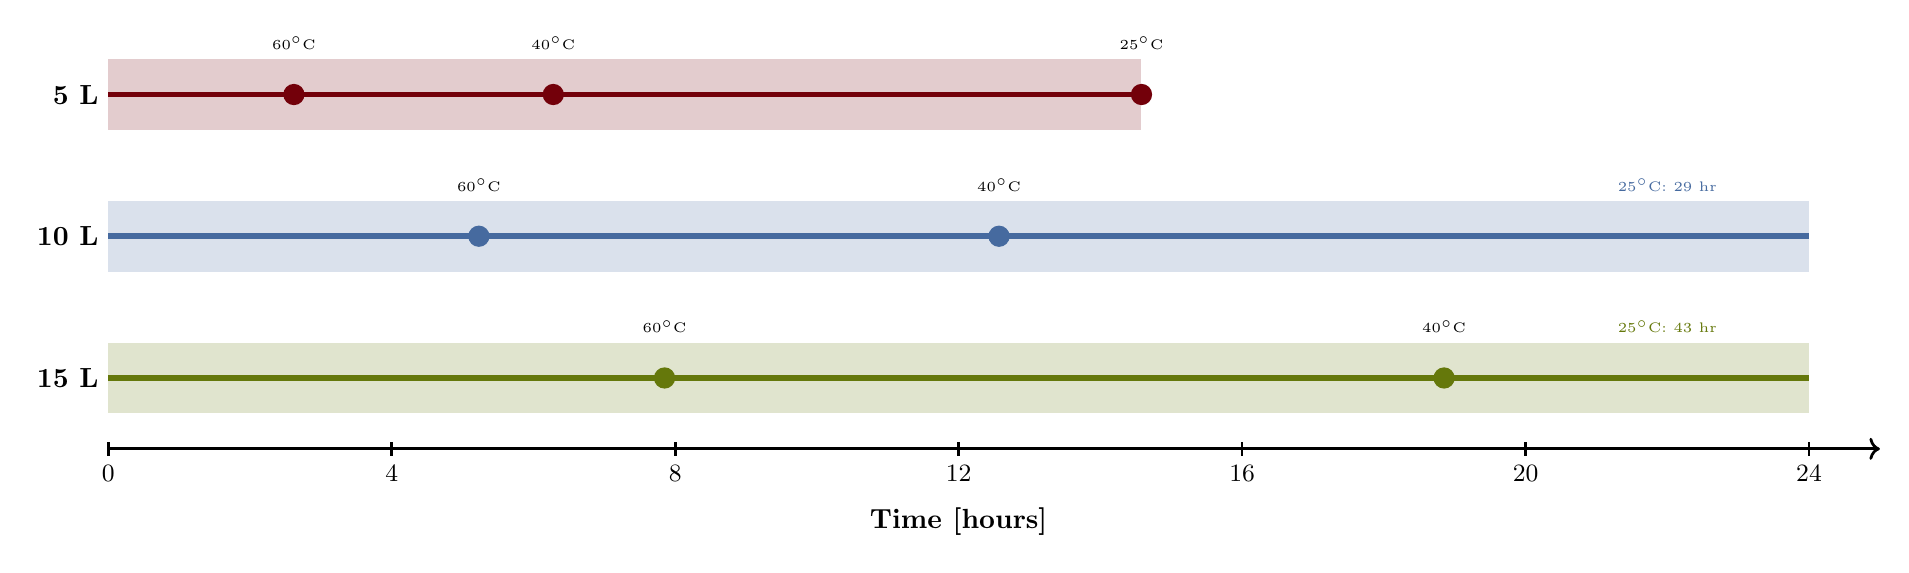
\begin{tikzpicture}[scale=0.9]
    % Timeline for 5 liters
    \fill[garnet!20] (0,4) rectangle (14.58,5);
    \draw[line width=2pt, garnet] (0,4.5) -- (14.58,4.5);
    \node[left, font=\bfseries] at (0,4.5) {5 L};

    % Markers
    \fill[garnet] (2.62,4.5) circle (0.15);
    \node[above, font=\tiny] at (2.62,5) {60\degC};
    \fill[garnet] (6.28,4.5) circle (0.15);
    \node[above, font=\tiny] at (6.28,5) {40\degC};
    \fill[garnet] (14.58,4.5) circle (0.15);
    \node[above, font=\tiny] at (14.58,5) {25\degC};

    % Timeline for 10 liters
    \fill[atlantic!20] (0,2) rectangle (24,3);
    \draw[line width=2pt, atlantic] (0,2.5) -- (24,2.5);
    \node[left, font=\bfseries] at (0,2.5) {10 L};

    \fill[atlantic] (5.23,2.5) circle (0.15);
    \node[above, font=\tiny] at (5.23,3) {60\degC};
    \fill[atlantic] (12.57,2.5) circle (0.15);
    \node[above, font=\tiny] at (12.57,3) {40\degC};
    \node[above, font=\tiny, atlantic] at (22,3) {25\degC: 29 hr};

    % Timeline for 15 liters
    \fill[horseshoe!20] (0,0) rectangle (24,1);
    \draw[line width=2pt, horseshoe] (0,0.5) -- (24,0.5);
    \node[left, font=\bfseries] at (0,0.5) {15 L};

    \fill[horseshoe] (7.85,0.5) circle (0.15);
    \node[above, font=\tiny] at (7.85,1) {60\degC};
    \fill[horseshoe] (18.85,0.5) circle (0.15);
    \node[above, font=\tiny] at (18.85,1) {40\degC};
    \node[above, font=\tiny, horseshoe] at (22,1) {25\degC: 43 hr};

    % Time axis
    \draw[->, line width=1pt] (0,-0.5) -- (25,-0.5);
    \foreach \x in {0,4,8,12,16,20,24} {
        \draw[line width=1pt] (\x,-0.6) -- (\x,-0.4);
        \node[below, font=\small] at (\x,-0.6) {\x};
    }
    \node[below, font=\bfseries] at (12,-1.2) {Time [hours]};

\end{tikzpicture}
\caption{Cooling timeline showing when water reaches key temperatures.}
\end{figure}

\section{Detailed Results}

\begin{table}[H]
\centering
\caption{Complete cooling timeline}
\begin{tabular}{l|ccc|ccc}
\toprule
& \multicolumn{3}{c|}{\textbf{Time to reach temperature}} & \multicolumn{3}{c}{\textbf{Temperature at time}} \\
\textbf{Volume} & 60\degC & 40\degC & 25\degC & 2 hr & 6 hr & 12 hr \\
\midrule
5 L & 2.6 hr & 6.3 hr & 14.6 hr & 69\degC & 44\degC & 29\degC \\
10 L & 5.2 hr & 12.6 hr & 29.2 hr & 78\degC & 58\degC & 42\degC \\
15 L & 7.9 hr & 18.9 hr & 43.5 hr & 81\degC & 65\degC & 50\degC \\
\bottomrule
\end{tabular}
\end{table}

\section{Physical Interpretation}

\subsection{Why the Exponential Decay?}

The cooling follows an exponential curve because:
\begin{equation}
    \frac{dT}{dt} = -\frac{T - T_\infty}{\tau}
\end{equation}

The rate of cooling is \textit{proportional to the temperature difference}. When hot, the water loses heat quickly; as it approaches ambient, the heat loss slows dramatically.

\subsection{Effect of Water Volume}

\begin{itemize}
    \item \textbf{Thermal capacitance} $C = mc_p$ increases linearly with mass
    \item \textbf{Heat loss rate} $Q = \Delta T / R$ is independent of mass (same at $t=0$)
    \item \textbf{Time constant} $\tau = RC$ increases linearly with mass
    \item \textbf{Result}: More water = slower cooling, proportionally longer times
\end{itemize}

\subsection{Practical Implications}

For keeping water hot:
\begin{itemize}
    \item 5 L of water drops below 60\degC{} in \textbf{2.6 hours}
    \item 10 L stays above 60\degC{} for \textbf{5.2 hours}
    \item 15 L stays above 60\degC{} for \textbf{7.9 hours}
\end{itemize}

The plywood enclosure provides reasonable insulation---initial heat loss is only $\sim$94 W compared to $\sim$600 W that would occur with direct exposure to air (no enclosure).

\section{Summary}

\begin{table}[H]
\centering
\caption{Key results summary}
\begin{tabular}{lccc}
\toprule
\textbf{Metric} & \textbf{5 L} & \textbf{10 L} & \textbf{15 L} \\
\midrule
Water mass & 5 kg & 10 kg & 15 kg \\
Thermal capacitance & 20.9 kJ/K & 41.9 kJ/K & 62.8 kJ/K \\
Time constant $\tau$ & 5.5 hr & 10.0 hr & 14.5 hr \\
Initial heat loss & 94 W & 94 W & 94 W \\
Time to 60\degC & 2.6 hr & 5.2 hr & 7.9 hr \\
Time to 40\degC & 6.3 hr & 12.6 hr & 18.9 hr \\
Time to 25\degC & 14.6 hr & 29.2 hr & 43.5 hr \\
\bottomrule
\end{tabular}
\end{table}

The time constant relationship is straightforward:
\begin{equation}
    \boxed{\tau \approx 1.1 \text{ hours per liter of water}}
\end{equation}

\end{document}
